\PassOptionsToPackage{unicode=true}{hyperref} % options for packages loaded elsewhere
\PassOptionsToPackage{hyphens}{url}
%
\documentclass[
]{article}
\usepackage{lmodern}
\usepackage{amssymb,amsmath}
\usepackage{ifxetex,ifluatex}
\ifnum 0\ifxetex 1\fi\ifluatex 1\fi=0 % if pdftex
  \usepackage[T1]{fontenc}
  \usepackage[utf8]{inputenc}
  \usepackage{textcomp} % provides euro and other symbols
\else % if luatex or xelatex
  \usepackage{unicode-math}
  \defaultfontfeatures{Scale=MatchLowercase}
  \defaultfontfeatures[\rmfamily]{Ligatures=TeX,Scale=1}
\fi
% use upquote if available, for straight quotes in verbatim environments
\IfFileExists{upquote.sty}{\usepackage{upquote}}{}
\IfFileExists{microtype.sty}{% use microtype if available
  \usepackage[]{microtype}
  \UseMicrotypeSet[protrusion]{basicmath} % disable protrusion for tt fonts
}{}
\makeatletter
\@ifundefined{KOMAClassName}{% if non-KOMA class
  \IfFileExists{parskip.sty}{%
    \usepackage{parskip}
  }{% else
    \setlength{\parindent}{0pt}
    \setlength{\parskip}{6pt plus 2pt minus 1pt}}
}{% if KOMA class
  \KOMAoptions{parskip=half}}
\makeatother
\usepackage{xcolor}
\IfFileExists{xurl.sty}{\usepackage{xurl}}{} % add URL line breaks if available
\IfFileExists{bookmark.sty}{\usepackage{bookmark}}{\usepackage{hyperref}}
\hypersetup{
  pdftitle={Scorigami!},
  pdfauthor={Austin Redmond},
  pdfborder={0 0 0},
  breaklinks=true}
\urlstyle{same}  % don't use monospace font for urls
\usepackage[margin=1in]{geometry}
\usepackage{color}
\usepackage{fancyvrb}
\newcommand{\VerbBar}{|}
\newcommand{\VERB}{\Verb[commandchars=\\\{\}]}
\DefineVerbatimEnvironment{Highlighting}{Verbatim}{commandchars=\\\{\}}
% Add ',fontsize=\small' for more characters per line
\usepackage{framed}
\definecolor{shadecolor}{RGB}{248,248,248}
\newenvironment{Shaded}{\begin{snugshade}}{\end{snugshade}}
\newcommand{\AlertTok}[1]{\textcolor[rgb]{0.94,0.16,0.16}{#1}}
\newcommand{\AnnotationTok}[1]{\textcolor[rgb]{0.56,0.35,0.01}{\textbf{\textit{#1}}}}
\newcommand{\AttributeTok}[1]{\textcolor[rgb]{0.77,0.63,0.00}{#1}}
\newcommand{\BaseNTok}[1]{\textcolor[rgb]{0.00,0.00,0.81}{#1}}
\newcommand{\BuiltInTok}[1]{#1}
\newcommand{\CharTok}[1]{\textcolor[rgb]{0.31,0.60,0.02}{#1}}
\newcommand{\CommentTok}[1]{\textcolor[rgb]{0.56,0.35,0.01}{\textit{#1}}}
\newcommand{\CommentVarTok}[1]{\textcolor[rgb]{0.56,0.35,0.01}{\textbf{\textit{#1}}}}
\newcommand{\ConstantTok}[1]{\textcolor[rgb]{0.00,0.00,0.00}{#1}}
\newcommand{\ControlFlowTok}[1]{\textcolor[rgb]{0.13,0.29,0.53}{\textbf{#1}}}
\newcommand{\DataTypeTok}[1]{\textcolor[rgb]{0.13,0.29,0.53}{#1}}
\newcommand{\DecValTok}[1]{\textcolor[rgb]{0.00,0.00,0.81}{#1}}
\newcommand{\DocumentationTok}[1]{\textcolor[rgb]{0.56,0.35,0.01}{\textbf{\textit{#1}}}}
\newcommand{\ErrorTok}[1]{\textcolor[rgb]{0.64,0.00,0.00}{\textbf{#1}}}
\newcommand{\ExtensionTok}[1]{#1}
\newcommand{\FloatTok}[1]{\textcolor[rgb]{0.00,0.00,0.81}{#1}}
\newcommand{\FunctionTok}[1]{\textcolor[rgb]{0.00,0.00,0.00}{#1}}
\newcommand{\ImportTok}[1]{#1}
\newcommand{\InformationTok}[1]{\textcolor[rgb]{0.56,0.35,0.01}{\textbf{\textit{#1}}}}
\newcommand{\KeywordTok}[1]{\textcolor[rgb]{0.13,0.29,0.53}{\textbf{#1}}}
\newcommand{\NormalTok}[1]{#1}
\newcommand{\OperatorTok}[1]{\textcolor[rgb]{0.81,0.36,0.00}{\textbf{#1}}}
\newcommand{\OtherTok}[1]{\textcolor[rgb]{0.56,0.35,0.01}{#1}}
\newcommand{\PreprocessorTok}[1]{\textcolor[rgb]{0.56,0.35,0.01}{\textit{#1}}}
\newcommand{\RegionMarkerTok}[1]{#1}
\newcommand{\SpecialCharTok}[1]{\textcolor[rgb]{0.00,0.00,0.00}{#1}}
\newcommand{\SpecialStringTok}[1]{\textcolor[rgb]{0.31,0.60,0.02}{#1}}
\newcommand{\StringTok}[1]{\textcolor[rgb]{0.31,0.60,0.02}{#1}}
\newcommand{\VariableTok}[1]{\textcolor[rgb]{0.00,0.00,0.00}{#1}}
\newcommand{\VerbatimStringTok}[1]{\textcolor[rgb]{0.31,0.60,0.02}{#1}}
\newcommand{\WarningTok}[1]{\textcolor[rgb]{0.56,0.35,0.01}{\textbf{\textit{#1}}}}
\usepackage{graphicx,grffile}
\makeatletter
\def\maxwidth{\ifdim\Gin@nat@width>\linewidth\linewidth\else\Gin@nat@width\fi}
\def\maxheight{\ifdim\Gin@nat@height>\textheight\textheight\else\Gin@nat@height\fi}
\makeatother
% Scale images if necessary, so that they will not overflow the page
% margins by default, and it is still possible to overwrite the defaults
% using explicit options in \includegraphics[width, height, ...]{}
\setkeys{Gin}{width=\maxwidth,height=\maxheight,keepaspectratio}
\setlength{\emergencystretch}{3em}  % prevent overfull lines
\providecommand{\tightlist}{%
  \setlength{\itemsep}{0pt}\setlength{\parskip}{0pt}}
\setcounter{secnumdepth}{-2}
% Redefines (sub)paragraphs to behave more like sections
\ifx\paragraph\undefined\else
  \let\oldparagraph\paragraph
  \renewcommand{\paragraph}[1]{\oldparagraph{#1}\mbox{}}
\fi
\ifx\subparagraph\undefined\else
  \let\oldsubparagraph\subparagraph
  \renewcommand{\subparagraph}[1]{\oldsubparagraph{#1}\mbox{}}
\fi

% set default figure placement to htbp
\makeatletter
\def\fps@figure{htbp}
\makeatother

% https://github.com/rstudio/rmarkdown/issues/337
\let\rmarkdownfootnote\footnote%
\def\footnote{\protect\rmarkdownfootnote}

% https://github.com/rstudio/rmarkdown/pull/252
\usepackage{titling}
\setlength{\droptitle}{-2em}

\pretitle{\vspace{\droptitle}\centering\huge}
\posttitle{\par}

\preauthor{\centering\large\emph}
\postauthor{\par}

\predate{\centering\large\emph}
\postdate{\par}

\title{Scorigami!}
\usepackage{etoolbox}
\makeatletter
\providecommand{\subtitle}[1]{% add subtitle to \maketitle
  \apptocmd{\@title}{\par {\large #1 \par}}{}{}
}
\makeatother
\subtitle{Using Markov Chains to Model Unique NFL Game Scores}
\author{Austin Redmond}
\date{4/12/2019}

\begin{document}
\maketitle

\hypertarget{introduction}{%
\section{Introduction}\label{introduction}}

\hypertarget{project-description-and-objectives}{%
\paragraph{Project Description and
Objectives}\label{project-description-and-objectives}}

Scorigami is the ``art of achieving a final score in an NFL game that
has never happened before'' (Bois). John Bois, an editor and
sportswriter at SB Nation (Colon), invented the term Scorigami in
December of 2016. The final score of an NFL game consists of the total
points scored by each of the two teams. There are six ways to score
points in an NFL game. The two most common ways to score are the 3-point
field goal and 7-point touchdown with a successful point-after-attempt.
The next three less common ways of scoring are the: 2-point safety;
6-point touchdown with a failed conversion; and the 8-point touchdown
with a successful 2-point conversion. The final and nearly impossible
way to score is the 1-point safety. The 1-point safety has never
occurred in the NFL but it is technically possible as ``a team making an
extra-point attempt {[}could{]} botch the play so badly, they would end
up in their own endzone, 98-yards away, and then get tackled in the
endzone'' (Nogle). The irregular distribution of scoring methods and the
relatively smaller sample size from a limited number of exactly 256
regular season and 12 postseason games per year means that many final
NFL scores that are possible have never actually happened. The website
\url{https://nflscorigami.com/} has a detailed representation of each
final score that has and has not occurred. The topic of this project is
related to using Markov Chains to project the probability of a unique
final NFL score (otherwise known as a Scorigami) happening given
parameters related to the the current score and how many quarters are
yet to occur in the game.

For this analysis each score, where one team is defined as the winning
team and the other is defined as the losing team, is considered a state
in the Markov Chain. The team that is winning may change from
quarter-to-quarter. In the data set, it is found that the largest amount
of points scored in a single quarter by a team is 31 points. Using this
information as a guideline, the upper bound of states will be a final
score of 124-124. The score of 124-124 is based off both teams scoring
31 points per quarter for all four quarters. The scenario described is
very extreme compared to actual events where: the highest number of
points scored in one game by one team is 73 and the highest number of
combined points scored by two teams is 105 points (NFL Scorigami).
States are recorded at the start of the game (where the score is always
equal to 0-0) and at the end of every quarter. Completing a quarter of
play will be considered one transition. Meaning each NFL game will have
exactly four transitions. Overtime will not be considered. If teams are
tied at the end of regulation, then the score will be considered final.
It can be assumed that the first, second, third, and fourth quarter have
the same or least similar scoring distributions. However, it is clear
that overtime, which has a limited number of scoring scenarios, has a
scoring distribution that is very different from the other quarters.

\hypertarget{literature-review}{%
\paragraph{Literature Review}\label{literature-review}}

No scholarly articles have been dedicated to the topic of scorigami.
There has been literature presented on the use of Markov chains to
predict outcomes in the NFL. For example, a Markov chain was used to
model the, at the time, new overtime rule system where the team that
wins the coin toss must score touchdown or concede safety for the
overtime period to end on the first possession. The transition matrix
was calculated using data on how a possession was most likely to end.
The conclusion found that new rule mitigated the advantage the team that
one the coin toss had in overtime (Jones).

Another article also used Markov chains to predict outcomes of NFL
overtimes. In the second article, the transition matrix is constructed
differently and simplified as certain ways of scoring were considered
negligible. For example, a successful safety was not considered as a
possible outcome because of its extremely low frequency (Leake). The
conclusions found in the second article, was very similar to the
conclusion found in the first article which justifies the simpler model
in the second article

\hypertarget{methodology}{%
\section{Methodology}\label{methodology}}

\hypertarget{my-library}{%
\subsubsection{My Library}\label{my-library}}

Call my libary in order to use functions stored in another r script. The
listed functions take the form.

game\_data(gameIds, gamePlayByPlay) initial\_distribution(states,
givenState) multi\_game\_scrape(seasons, types, weeks = NULL, teams =
NULL) multi\_game\_play\_by\_play(gameIDs)
points\_scored\_frequency(gameData)
points\_scored\_observations(pointsScoredFrequency)
scorigami\_probability(stateProbabilityDistribution, missingStates)
state\_probability\_distribution(initialDistribution, transitionMarix,
quarters remaining) transition\_matrix\_one(states,
pointsScoredFrequency) transition\_matrix\_two(states,
pointsScoredFrequency)

\begin{Shaded}
\begin{Highlighting}[]
\KeywordTok{source}\NormalTok{(}\StringTok{"~/GitHub/ScorigamiMC/ScorigamiMCLibrary.R"}\NormalTok{)}
\end{Highlighting}
\end{Shaded}

\hypertarget{data-scraping}{%
\subsubsection{Data Scraping}\label{data-scraping}}

\hypertarget{install-nflscrapr}{%
\paragraph{Install nflscrapR}\label{install-nflscrapr}}

The data for this analysis was collected using nflscrapR which is an R
package that is used to ``utilize and analyze data from the National
Football League (NFL) API'' (How). It is necessary to install it in
order to scrape data pertaining to NFL box scores. The nflscrapR package
can be found at \url{https://github.com/maksimhorowitz/nflscrapR}. The
devtools package can install R packages hosted on Github.

\begin{Shaded}
\begin{Highlighting}[]
\CommentTok{#Load the devtools library to install packages found on github.}
\KeywordTok{library}\NormalTok{(devtools)}

\CommentTok{#Install nflscrapR from the designated Github repository.}
\NormalTok{devtools}\OperatorTok{::}\KeywordTok{install_github}\NormalTok{(}\DataTypeTok{repo =} \StringTok{"maksimhorowitz/nflscrapR"}\NormalTok{)}
\end{Highlighting}
\end{Shaded}

\hypertarget{scrape-individual-games}{%
\paragraph{Scrape Individual Games}\label{scrape-individual-games}}

Ten years worth of regular and post season games between 2009 and 2018
are collected for analysis. During this period, 2560 regular season
games and 120 postseason games were played in the NFL. Each observation
represents a unique game. Each game has 10 variables that record: a
unique game ID; the game's type which indicates whether the game is a
regular season or postseason game; the home team; the away team; the
week of the season that the game was played; the score of the home team
at the end of the game; the score of the away team at the end of the
game; a unique url associated with the game; and the status of the game
indicating whether the game is finished or ongoing.

\begin{Shaded}
\begin{Highlighting}[]
\CommentTok{#Scrape all regular and post season game ids from 2009 to 2018.}
\CommentTok{#scrapedGameIDs <- multi_scrape_game_ids(2009:2018, c("reg", "post")) #This is the original line.}
\KeywordTok{load}\NormalTok{(}\StringTok{"scrapedGameIDs.Rda"}\NormalTok{)}

\CommentTok{#Save scraped game ids to file.}
\KeywordTok{save}\NormalTok{(scrapedGameIDs, }\DataTypeTok{file =} \StringTok{"scrapedGameIDs.Rda"}\NormalTok{)}

\CommentTok{#dplyr is used to select or deselect certain variables for in a data set. }
\KeywordTok{library}\NormalTok{(dplyr)}

\CommentTok{#Display the first six observations.}
\KeywordTok{head}\NormalTok{(}\KeywordTok{select}\NormalTok{(scrapedGameIDs, }\OperatorTok{-}\KeywordTok{c}\NormalTok{(}\StringTok{"game_url"}\NormalTok{, }\StringTok{"state_of_game"}\NormalTok{)))}
\end{Highlighting}
\end{Shaded}

\begin{verbatim}
##   type    game_id home_team away_team week season home_score away_score
## 1  reg 2009091000       PIT       TEN    1   2009         13         10
## 2  reg 2009091304       CLE       MIN    1   2009         20         34
## 3  reg 2009091307        NO       DET    1   2009         45         27
## 4  reg 2009091308        TB       DAL    1   2009         21         34
## 5  reg 2009091305       HOU       NYJ    1   2009          7         24
## 6  reg 2009091306       IND       JAC    1   2009         14         12
\end{verbatim}

\hypertarget{scrape-game-play-by-play}{%
\paragraph{Scrape Game Play-by-Play}\label{scrape-game-play-by-play}}

All previously scraped game IDs collected from 2009 to 2018 are used to
get play-by-play data. Each observation represents a unique play. The
only variables collected from the play-by-play were; the unique game id;
the home team, the away team; the quarter the play happened; the home
score; and the away score. All other variables were discarded. For this
analysis, it is necessary to record the scores at the end of each of the
4 quarters because that is considered a state. All observations that are
not indicated as resulting in the quarter ending are also discarded.
This action is executed by conditioning the data on a variable that
indicates whether the quarter ends immediately after the play occurs.

\begin{Shaded}
\begin{Highlighting}[]
\CommentTok{#Load the scraped game ids data frame from file.}
\KeywordTok{load}\NormalTok{(}\StringTok{"scrapedGameIDs.Rda"}\NormalTok{)}

\CommentTok{#Scrape play-by-play data of all selected games.}
\CommentTok{#scrapedGamePlayByPlay <- multi_scrape_game_play_by_play(scrapedGameIDs)}
\KeywordTok{load}\NormalTok{(}\StringTok{"scrapedGamePlayByPlay.Rda"}\NormalTok{)}

\CommentTok{#Save scraped game play-by-play data to file.}
\KeywordTok{save}\NormalTok{(scrapedGamePlayByPlay, }\DataTypeTok{file =} \StringTok{"scrapedGamePlayByPlay.Rda"}\NormalTok{)}

\CommentTok{#Display the first six observations.}
\KeywordTok{head}\NormalTok{(scrapedGamePlayByPlay)}
\end{Highlighting}
\end{Shaded}

\begin{verbatim}
## # A tibble: 6 x 6
##   game_id    home_team away_team   qtr total_home_score total_away_score
##   <chr>      <chr>     <chr>     <dbl>            <dbl>            <dbl>
## 1 2009091000 PIT       TEN           1                0                0
## 2 2009091000 PIT       TEN           3                7                7
## 3 2009091000 PIT       TEN           4               10               10
## 4 2009091304 CLE       MIN           1                3                3
## 5 2009091304 CLE       MIN           2               12               10
## 6 2009091304 CLE       MIN           3               12               24
\end{verbatim}

\hypertarget{combine-data-sets}{%
\paragraph{Combine Data Sets}\label{combine-data-sets}}

The two data sets are merged together so that each observation in the
merged data set will represent one game. The structure of the merged
data set is the same as the scraped individual game data set. The score
at the end of each quarter, which is information found in the
play-by-play data set, is added to each observation in the merged data
set.

\begin{Shaded}
\begin{Highlighting}[]
\CommentTok{#Load both scraped datasets.}
\KeywordTok{load}\NormalTok{(}\StringTok{"scrapedGameIDs.Rda"}\NormalTok{)}
\KeywordTok{load}\NormalTok{(}\StringTok{"scrapedGamePlayByPlay.Rda"}\NormalTok{)}

\CommentTok{#Merge the scaped game Id dataset and the scraped game play-by-play data set.}
\NormalTok{gameData <-}\StringTok{ }\KeywordTok{game_data}\NormalTok{(scrapedGameIDs, scrapedGamePlayByPlay)}

\CommentTok{#Save merged game data to file.}
\KeywordTok{save}\NormalTok{(gameData, }\DataTypeTok{file =} \StringTok{"gameData.Rda"}\NormalTok{)}
\end{Highlighting}
\end{Shaded}

The first six observations demonstrate the limitations of how the data
was originally recorded. Some plays that were the last play of the
quarter were not properly recorded as such. When this error in the NFL's
records occurs, an NA will be recorded in the data set. It is not ideal
to have missing data. However it is possible to proceed to the
construction of the points scored distributions. If the score is missing
at the end of one quarter for any game, there is still 2 or 3 quarters
where the amount of points scored is known. That information can still
be used to construct the points scored distributions.

\begin{Shaded}
\begin{Highlighting}[]
\CommentTok{#Load the merged data set.}
\KeywordTok{load}\NormalTok{(}\StringTok{"gameData.Rda"}\NormalTok{)}

\CommentTok{#Display the first six observations.}
\KeywordTok{head}\NormalTok{(gameData)}
\end{Highlighting}
\end{Shaded}

\begin{verbatim}
##      game_id home_team away_team qtr1_home_score qtr1_away_score
## 1 2009091000       PIT       TEN               0               0
## 2 2009091304       CLE       MIN               3               3
## 3 2009091307        NO       DET              14               3
## 4 2009091308        TB       DAL               0               6
## 5 2009091305       HOU       NYJ               0               3
## 6 2009091306       IND       JAC               0               0
##   qtr2_home_score qtr2_away_score qtr3_home_score qtr3_away_score
## 1            <NA>            <NA>               7               7
## 2              12              10              12              24
## 3              28              10              38              26
## 4            <NA>            <NA>               7              20
## 5               0              10               0              17
## 6            <NA>            <NA>              14               6
##   qtr4_home_score qtr4_away_score final_home_score final_away_score
## 1              10              10               13               10
## 2              19              34               20               34
## 3              45              26               45               27
## 4              21              34               21               34
## 5               6              24                7               24
## 6              14              12               14               12
\end{verbatim}

\hypertarget{the-markov-chain-representation}{%
\subsubsection{The Markov Chain
Representation}\label{the-markov-chain-representation}}

\hypertarget{possible-states}{%
\paragraph{Possible States}\label{possible-states}}

As described before, each state will include two scores. The first score
is the winning team's total points and the second score is the losing
team's total points. The winning and losing teams may be tied but (for
this analysis) it is considered trivial which actual team is considered
the winning and losing team. The minimum points scored by a team in one
quarter is 0 points for the data set. On the other hand, the maximum
points scored in one quarter by a team is 31 for the data set. Although
unlikely, we consider the probability of a team scoring 31 points every
quarter to have a non-zero probability. In an NFL game there are four
steps representing a quarter that is played. By definition the final
score of the winning team is always greater than or equal the final
score of the losing team. The possible states are:

\{``w-l''\textbar{}w and l are elements of the set of integers between 0
and 124, w \textgreater{}= l\}

\begin{Shaded}
\begin{Highlighting}[]
\CommentTok{#Create a vector of states with the first element being the score "0-0".}
\NormalTok{states <-}\StringTok{ }\KeywordTok{c}\NormalTok{(}\StringTok{"0-0"}\NormalTok{)}

\CommentTok{#Loop through each of the possible states,"w-l".}
\CommentTok{#Add the result to the states vector.}
\ControlFlowTok{for}\NormalTok{(w }\ControlFlowTok{in} \DecValTok{1}\OperatorTok{:}\DecValTok{124}\NormalTok{) \{}
  \ControlFlowTok{for}\NormalTok{(l }\ControlFlowTok{in} \DecValTok{0}\OperatorTok{:}\NormalTok{w) \{}
\NormalTok{    states[[}\KeywordTok{length}\NormalTok{(states)}\OperatorTok{+}\DecValTok{1}\NormalTok{]] <-}\StringTok{ }\KeywordTok{paste}\NormalTok{(w,l, }\DataTypeTok{sep =}\StringTok{"-"}\NormalTok{)}
\NormalTok{  \}}
\NormalTok{\}}

\CommentTok{#Save the states vector to file.}
\KeywordTok{save}\NormalTok{(states, }\DataTypeTok{file=}\StringTok{"states.Rda"}\NormalTok{)}
\end{Highlighting}
\end{Shaded}

\hypertarget{missing-states}{%
\paragraph{Missing States}\label{missing-states}}

\begin{figure}
\centering
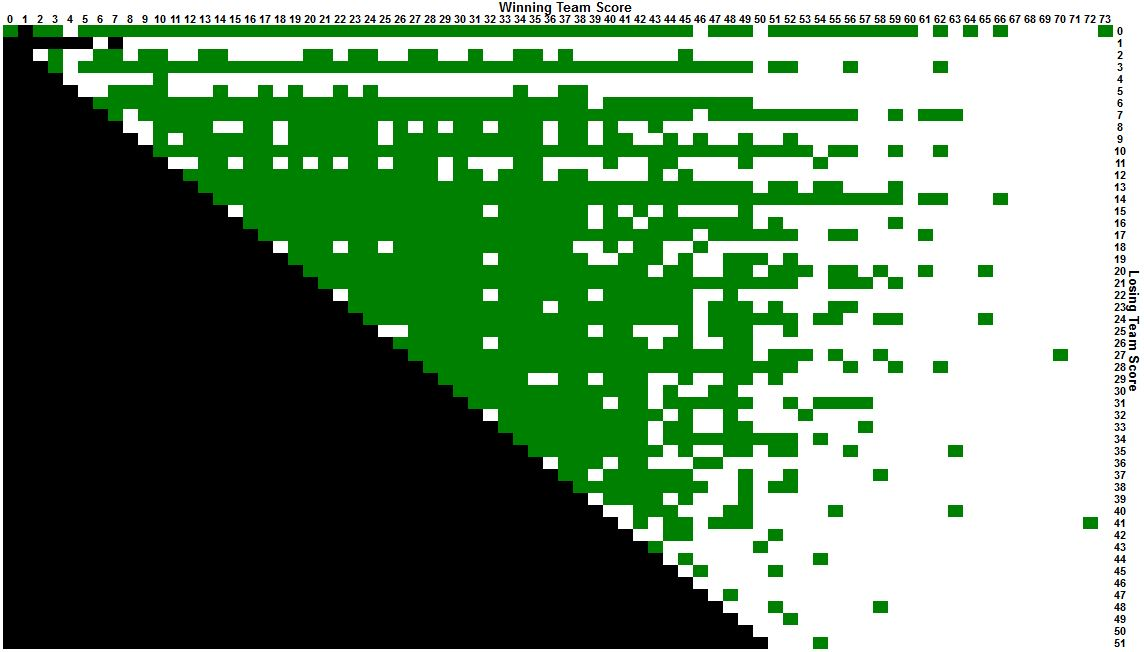
\includegraphics{https://www.ualberta.ca/~aredmond/nflscorigami.JPG}
\caption{Scorigami Matrix Found at www.nflscorigami.com}
\end{figure}

The diagram above illustrates most of the possible states that are
considered in this analysis. Black squares are not considered possible
states. Green squares indicate that the final score has occurred at
least once. The white squares represent a final score that has never
occurred before. A scorigami occurs whenever a unique final score occurs
for the first time. Pro football reference provides a data set including
all the missing final scores that have never occurred before.

\begin{Shaded}
\begin{Highlighting}[]
\CommentTok{#Load the missing score data from csv.}
\NormalTok{missingScoresData <-}\StringTok{ }\KeywordTok{read.csv}\NormalTok{(}\DataTypeTok{file=}\StringTok{"missingScores.csv"}\NormalTok{, }\DataTypeTok{header =} \OtherTok{TRUE}\NormalTok{, }\DataTypeTok{sep =} \StringTok{","}\NormalTok{)}

\CommentTok{#The all missing states between "2-2" and "70-70".}
\NormalTok{missingStates <-}\StringTok{ }\KeywordTok{as.character}\NormalTok{(missingScoresData}\OperatorTok{$}\NormalTok{Score)}

\CommentTok{#Add each state between "71-0" and "124-124"}
\ControlFlowTok{for}\NormalTok{(w }\ControlFlowTok{in} \DecValTok{71}\OperatorTok{:}\DecValTok{124}\NormalTok{) \{}
  \ControlFlowTok{for}\NormalTok{(l }\ControlFlowTok{in} \DecValTok{0}\OperatorTok{:}\NormalTok{w) \{}
\NormalTok{    missingStates[[}\KeywordTok{length}\NormalTok{(missingStates)}\OperatorTok{+}\DecValTok{1}\NormalTok{]] <-}\StringTok{ }\KeywordTok{paste}\NormalTok{(w,l, }\DataTypeTok{sep=}\StringTok{"-"}\NormalTok{)}
\NormalTok{  \}}
\NormalTok{\}}

\CommentTok{#Remove the states "72-41" and "73-0" because they have occurred before.}
\NormalTok{missingStates <-}\StringTok{ }\KeywordTok{setdiff}\NormalTok{(missingStates, }\KeywordTok{c}\NormalTok{(}\StringTok{"72-41"}\NormalTok{, }\StringTok{"73-0"}\NormalTok{))}

\KeywordTok{save}\NormalTok{(missingStates, }\DataTypeTok{file=}\StringTok{"missingStates.Rda"}\NormalTok{)}
\end{Highlighting}
\end{Shaded}

\hypertarget{initial-distribution}{%
\paragraph{Initial Distribution}\label{initial-distribution}}

The initial distribution defines the probability of each state at the
start. In the context of an NFL game, only one score can exist at a
time. As every game starts with a score of 0 to 0, a standard initial
distribution will have 100\% probability of being state ``0-0''. It is
possible to start the projection at other points in time such as the
start of the second, third, and fourth quarters. If this is the case,
the number of transitions will need to reflect the different point in
time.

\begin{Shaded}
\begin{Highlighting}[]
\KeywordTok{load}\NormalTok{(}\StringTok{"states.Rda"}\NormalTok{)}

\NormalTok{standardInitialDistribution <-}\StringTok{ }\KeywordTok{initial_distribution}\NormalTok{(states, }\StringTok{"0-0"}\NormalTok{)}

\KeywordTok{save}\NormalTok{(standardInitialDistribution, }\DataTypeTok{file=}\StringTok{"standardInitialDistribution.Rda"}\NormalTok{)}
\end{Highlighting}
\end{Shaded}

\hypertarget{points-scored-distributions}{%
\paragraph{Points Scored
Distributions}\label{points-scored-distributions}}

The first step in constructing the transition matrices is to determine
the distribution of points scored by a team in a quarter. The winning
team in a given quarter is defined as the team that is winning the game
at the start of the quarter. While the losing team in a given quarter is
defined as the team that is losing the game at the start of the quarter.
If the teams are tied at the start of the quarter, then the team that
scored more points in that quarter is considered the winning team. The
winning team and losing team can change from quarter-to-quarter.

The graph below plots the points scored by the winning team and the
losing team in one quarter for every quarter recorded in the data set. A
single observation includes the points scored from both teams. The
x-axis shows the quantity of points scored by the winning team in one
quarter. The winning team has scored anywhere from 0 to 31 points. The
x-axis shows the quantity of points scored by the losing team in one
quarter. The losing team has scored anywhere from 0 to 28 points.

The color of each cell in the grid represents the amount of observations
where the winning team and the losing team specifically scored that many
points in a quarter. This means that we are treating the scores of the
winning team and losing team as dependent. There are 10 colors
representing ten bins. The first bin has a black color and each bin
thereafter is a lighter color. The tenth bin therefore is yellow. Any
cell that is white has no observations. The size of the bins were
determined so that they contain roughly the same number of observations.
They are as follows: bin 1 (1 observation), bin 2 (2 observations), bin
3 (3 observations), bin 4 (4-5 observations), bin 5 (6-9 observations),
bin 6 (10-14 observations), bin 7 (14-50 observations), bin 8 (51-100
observations), bin 9 (101-150 observations), and bin 10 (151
observations or greater).

\begin{Shaded}
\begin{Highlighting}[]
\CommentTok{#Load the game data.}
\KeywordTok{load}\NormalTok{(}\StringTok{"gameData.Rda"}\NormalTok{)}

\CommentTok{#Get the frequency of how many points are scored by the the two teams within the game data. This functiomn will return a matrix.}
\NormalTok{pointsScoredFrequency <-}\StringTok{ }\KeywordTok{points_scored_frequency}\NormalTok{(gameData)}

\CommentTok{#Save the points scored frequency matrix to file.}
\KeywordTok{save}\NormalTok{(pointsScoredFrequency, }\DataTypeTok{file=}\StringTok{"pointsScoredFrequency.Rda"}\NormalTok{)}

\CommentTok{#Load the plot.matrix and viridis libraries to create a graph of the points scored frequency matrix.}
\KeywordTok{library}\NormalTok{(plot.matrix)}
\KeywordTok{library}\NormalTok{(viridis)}

\CommentTok{#Plot the points scored frequency matrix,}
\NormalTok{x <-}\StringTok{ }\NormalTok{pointsScoredFrequency}
\NormalTok{x[x}\OperatorTok{==}\DecValTok{0}\NormalTok{] <-}\StringTok{ }\OtherTok{NA}
\KeywordTok{plot}\NormalTok{(x, }\DataTypeTok{breaks=}\KeywordTok{c}\NormalTok{(}\DecValTok{0}\NormalTok{,}\DecValTok{1}\NormalTok{,}\DecValTok{2}\NormalTok{,}\DecValTok{3}\NormalTok{,}\DecValTok{5}\NormalTok{,}\DecValTok{9}\NormalTok{,}\DecValTok{14}\NormalTok{,}\DecValTok{50}\NormalTok{,}\DecValTok{100}\NormalTok{,}\DecValTok{150}\NormalTok{,}\DecValTok{1000}\NormalTok{),}\DataTypeTok{col =}\NormalTok{ magma, }\DataTypeTok{main=}\StringTok{"Points Scored Frequency Matrix"}\NormalTok{, }\DataTypeTok{xlab =} \StringTok{"Winning Team Points Scored in One Quarter"}\NormalTok{, }\DataTypeTok{ylab =} \StringTok{"Losing Team Points Scored in One Quarter"}\NormalTok{)}
\end{Highlighting}
\end{Shaded}

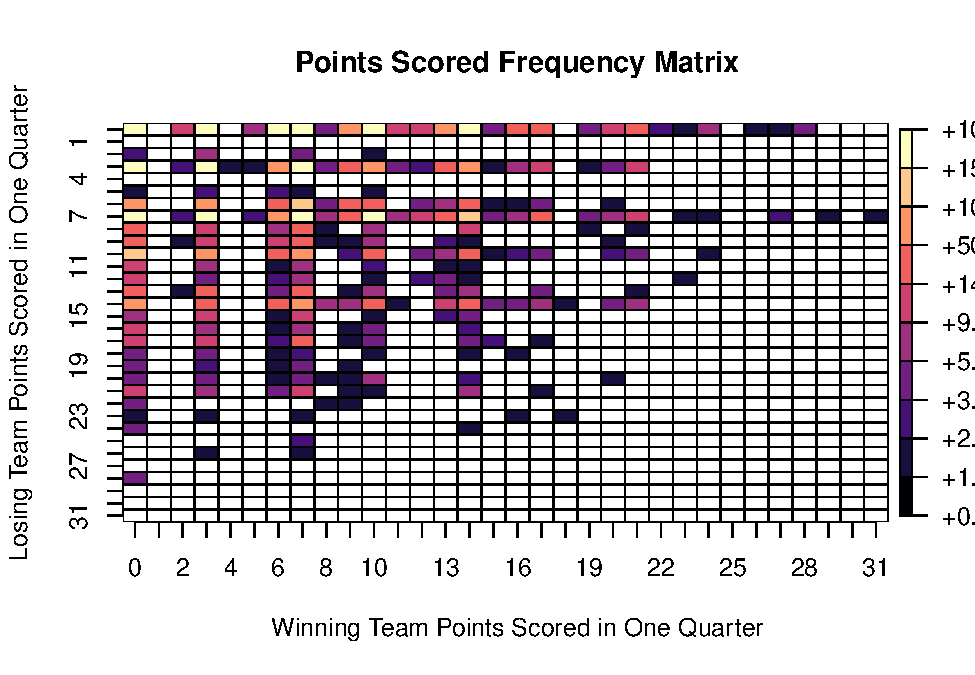
\includegraphics{ScorigamiMC_files/figure-latex/Points Scored Frequency Matrix-1.pdf}

When observing the graph, it is clear that many combinations of scores
have not occurred in period of 2009 to 2018. Given the yellow cells, it
is evident that the most common combinations of scores are those where
both teams have a score that is a linear transformation of {[}3x+7y{]}
where x and y are 0, 1, or 2. This result is intuitive given that: first
the 3-point field goal and the 7-point touchdown with successful
point-after attempt are the most common ways to score and second it is
difficult to score on 3 or more drives in a quarter as each quarter is
time constrained to 15 minutes of game time. Scores that are only
possible using at least one 2-point safety and/or 8-point touchdown are
very unlikely to occur. A few examples of unlikely amounts of points
scored in a quarter are 2, 4, 5, 8, 11, and 15 to name a few. Columns or
rows featuring a rare score like those mentioned are likely to be mostly
white, black, or darker shades of purple.

The amount of points scored by the winning and losing teams may or may
not be independent. Only one team can have possession of the ball at any
given point in time. It would be expected that a higher score by one
team means that the other team has less position time. However, it is
difficult to claim that the chance of scoring a rare score in a quarter
is more or less likely based on the other team also scoring a rare
score. The graph above shows many combinations of scores as impossible
(the cell is white) when they are merely improbable. The sample of only
includes 6691 different quarters. Given a larger sample size it is
possible for more combinations to occur. Given this it is appropriate to
build two different transition matrices based on two different
assumptions.

Assumption \#1: The points scored by each team is dependent. We should
consider the points scored in the same quarter of the same game as
dependent on each other.

Assumption \#2: The points scored by each team is independent. We should
consider distribution of points scored by the winning team and the
losing team as two different distributions that exist separately.

\begin{Shaded}
\begin{Highlighting}[]
\CommentTok{#Get the individual observations from the points scored frequency mattrix.}
\NormalTok{pointsScoredObservations <-}\StringTok{ }\KeywordTok{points_scored_observations}\NormalTok{(pointsScoredFrequency)}

\CommentTok{#Save the individual points scored matrix to file.}
\KeywordTok{save}\NormalTok{(pointsScoredObservations, }\DataTypeTok{file=}\StringTok{"pointsScoredObservations.Rda"}\NormalTok{)}

\CommentTok{#Load the ggplot2 library to creat a histogram with two distributions.}
\KeywordTok{library}\NormalTok{(ggplot2)}

\CommentTok{#Create a histogram that graphs the winning team points scored and the losing team points scored separately.}
\KeywordTok{ggplot}\NormalTok{() }\OperatorTok{+}\StringTok{ }
\StringTok{  }\KeywordTok{geom_histogram}\NormalTok{(}\KeywordTok{aes}\NormalTok{(}\DataTypeTok{x =}\NormalTok{ pointsScoredObservations}\OperatorTok{$}\NormalTok{losing_team_points_scored, }\DataTypeTok{fill =} \StringTok{"r"}\NormalTok{), }\DataTypeTok{alpha =} \FloatTok{0.3}\NormalTok{, }\DataTypeTok{bins =} \DecValTok{31}\NormalTok{) }\OperatorTok{+}
\StringTok{  }\KeywordTok{geom_histogram}\NormalTok{(}\KeywordTok{aes}\NormalTok{(}\DataTypeTok{x =}\NormalTok{ pointsScoredObservations}\OperatorTok{$}\NormalTok{winning_team_points_scored, }\DataTypeTok{fill =} \StringTok{"b"}\NormalTok{), }\DataTypeTok{alpha =} \FloatTok{0.3}\NormalTok{, }\DataTypeTok{bins =} \DecValTok{31}\NormalTok{) }\OperatorTok{+}
\StringTok{  }\KeywordTok{scale_colour_manual}\NormalTok{(}\DataTypeTok{name =}\StringTok{"Histograms of Points Scored"}\NormalTok{, }\DataTypeTok{values =} \KeywordTok{c}\NormalTok{(}\StringTok{"r"}\NormalTok{ =}\StringTok{ "red"}\NormalTok{, }\StringTok{"b"}\NormalTok{ =}\StringTok{ "blue"}\NormalTok{), }\DataTypeTok{labels=}\KeywordTok{c}\NormalTok{(}\StringTok{"b"}\NormalTok{ =}\StringTok{ "Winning Team"}\NormalTok{, }\StringTok{"r"}\NormalTok{ =}\StringTok{ "Losing Team"}\NormalTok{)) }\OperatorTok{+}
\StringTok{  }\KeywordTok{scale_fill_manual}\NormalTok{(}\DataTypeTok{name =}\StringTok{"Legend"}\NormalTok{, }\DataTypeTok{values =} \KeywordTok{c}\NormalTok{(}\StringTok{"r"}\NormalTok{ =}\StringTok{ "red"}\NormalTok{, }\StringTok{"b"}\NormalTok{ =}\StringTok{ "blue"}\NormalTok{), }\DataTypeTok{labels=}\KeywordTok{c}\NormalTok{(}\StringTok{"b"}\NormalTok{ =}\StringTok{ "Winning Team"}\NormalTok{, }\StringTok{"r"}\NormalTok{ =}\StringTok{ "Losing Team"}\NormalTok{))}\OperatorTok{+}
\StringTok{  }\KeywordTok{labs}\NormalTok{(}\DataTypeTok{title =} \StringTok{"Histograms of Points Scored"}\NormalTok{, }\DataTypeTok{x =} \StringTok{"Points Scored in One Quarter"}\NormalTok{, }\DataTypeTok{y =} \StringTok{"Frequency"}\NormalTok{)}
\end{Highlighting}
\end{Shaded}

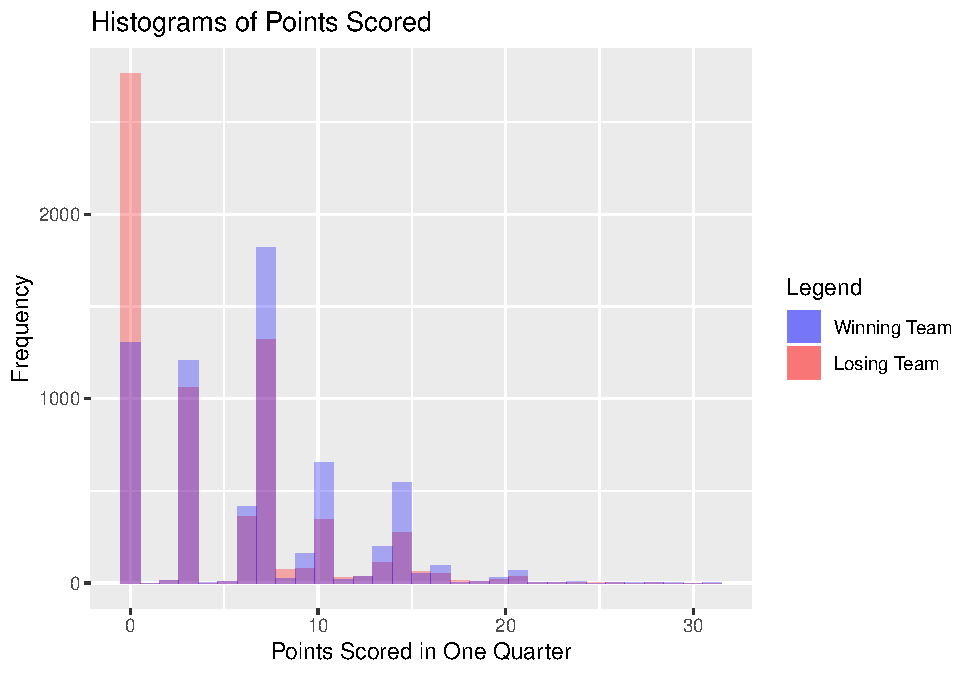
\includegraphics{ScorigamiMC_files/figure-latex/Get Points Scored Distributions-1.pdf}

The histogram above represents the distributions of points scored by
each of the winning and losing teams. The winning teams are designated
with the color blue and the losing teams are designated with the color
red. It can be observed that the distributions are not normal. The same
common scores (0,3,7,10\ldots{}) and rare scores (2,4,5, 8\ldots{})
noted previously are also displayed convincingly in this histogram. In
terms of differences between the histograms. It can be observed that the
losing teams score 0 points in a given quarter way more more often than
the winning teams. If a team is losing at the start of a quarter, it is
not surprising that they are more likely to score 0 points in that
quarter because they are probably a worse offensive team. For the most
part, the winning teams have more observations where the points scored
is above 3 or above. However, there are three counter-examples that are
interesting. When the points scored is 8, 11, or 15, there are more
observations for the losing teams. If a team is losing, then they will
play riskier in order to catch up to the team that is winning. Riskier
play will result in teams that are more willing to go for a 2-point
conversion attempt. If they are successful, then their points scored for
that quarter will be a linear transformation of {[}3x+7y+8z{]} where 8
is equal to 1. The scores of 8, 11, and 15 are all likely in the
described scenario.

\hypertarget{transiton-matrix}{%
\paragraph{Transiton Matrix}\label{transiton-matrix}}

The transition matrix is constructed according to the two assumptions
outlined in the previous section. They were:

Assumption \#1: The points scored by each team is dependent. We should
consider the points scored in the same quarter of the same game as
dependent on each other.

Assumption \#2: The points scored by each team is independent. We should
consider distribution of points scored by the winning team and the
losing team as two different distributions that exist separately.

For transition matrix one, the number of observations for each
combination of points scored by the winning and losing teams is divided
by the total number of observations. The resulting quotient is
considered the relative frequency for that combination of points. If it
is possible to get from one state to another state, there are usually
two ways to get there. Either the winning team remained the winning team
or the losing team became the winning team. The probability of both
scenarios is calculated by adding the relevant points scored relative
frequencies. All states where the winning team scored 94 or more points
are considered an absorbing state. The justification for this decision
is that it should not be possible to score 94 points in less than four
quarters. This is based on the most points scored in a quarter being 31
points.

For transition matrix two, the number of observations for each row and
column is divided by the total number of observations. The resulting
quotients are considered the relative frequency for: the points scored
by the winning team and the points scored by the losing team. Again if
it is possible to get from one state to another state, there are usually
two ways to get there. Either the winning team remained the winning team
or the losing team became the winning team. The probability of the
points scored by the winning team and the probability of the points
scored by the losing team are assumed to be independent so they are
directly multiplied by each other to calculate the probability of both
events occurring. The scenarios that go from one state to the other are
added together. All states where the winning or losing team scored 94 or
more points are considered an absorbing state. The justification here is
the same as the justification for the first transition matrix.

\begin{Shaded}
\begin{Highlighting}[]
\CommentTok{#Load the states vector and the points scored frequency matrix.}
\KeywordTok{load}\NormalTok{(}\StringTok{"states.Rda"}\NormalTok{)}
\KeywordTok{load}\NormalTok{(}\StringTok{"pointsScoredFrequency.Rda"}\NormalTok{)}

\CommentTok{#Construct the first matrix based on assumption #1.}
\CommentTok{#transitionMatrixOne <- transition_matrix_one(states, pointsScoredFrequency) #This is the original line.}
\KeywordTok{load}\NormalTok{(}\StringTok{"transitionMatrixOne.Rda"}\NormalTok{)}

\CommentTok{#Save the first transition matrix to file.}
\KeywordTok{save}\NormalTok{(transitionMatrixOne, }\DataTypeTok{file=}\StringTok{"transitionMatrixOne.Rda"}\NormalTok{)}

\CommentTok{#Construct the second matrix based on assumption #2}
\CommentTok{#transitionMatrixTwo <- transition_matrix_two(states, pointsScoredFrequency) #This is the original line.}
\KeywordTok{load}\NormalTok{(}\StringTok{"transitionMatrixTwo.Rda"}\NormalTok{)}

\CommentTok{#Save the second transition matrix to file.}
\KeywordTok{save}\NormalTok{(transitionMatrixTwo, }\DataTypeTok{file=}\StringTok{"transitionMatrixTwo.Rda"}\NormalTok{)}
\end{Highlighting}
\end{Shaded}

\hypertarget{results}{%
\section{Results}\label{results}}

\hypertarget{using-markov-chains-to-model-unique-nfl-game-scores}{%
\subsubsection{Using Markov Chains to Model Unique NFL Game
Scores}\label{using-markov-chains-to-model-unique-nfl-game-scores}}

\hypertarget{state-probability-distributions-with-standard-initial-distributions}{%
\paragraph{State Probability Distributions with Standard Initial
Distributions}\label{state-probability-distributions-with-standard-initial-distributions}}

The state probability distribution is calculated using the initial
distribution, the transition matrix, and the number of steps (which are
also known as the quarters to be played). The formula is written as:

transpose(transitionMatrix\^{}steps)*initialDistribution

To calculate how often a Scorigami should occur in the average NFL game,
the two transition matrices are tried, the standard initial distribution
is used, and 4 steps are considered. The resulting state probability
distribution is then conditioned so that only states that have never
occurred before are considered. The sum of the remaining elements are
calculated to find the probability of a scorigami.

\begin{Shaded}
\begin{Highlighting}[]
\CommentTok{#Load the standard origin Matrix which designates that every game begins with a score of "0-0" with 100% probability.}
\KeywordTok{load}\NormalTok{(}\StringTok{"standardInitialDistribution.Rda"}\NormalTok{)}

\CommentTok{#Load the first transition matrix.}
\KeywordTok{load}\NormalTok{(}\StringTok{"transitionMatrixOne.Rda"}\NormalTok{)}

\CommentTok{#Calculate the state probability distribution after the 4 transitions.}
\CommentTok{#stateProbabilityDistributionOne <- state_probability_distribution(standardInitialDistribution, transitionMatrixOne, 4) #This is the original line.}
\KeywordTok{load}\NormalTok{(}\StringTok{"stateProbabilityDistributionOne.Rda"}\NormalTok{)}

\CommentTok{#Save state probability distribution to file.}
\KeywordTok{save}\NormalTok{(stateProbabilityDistributionOne, }\DataTypeTok{file =} \StringTok{"stateProbabilityDistributionOne.Rda"}\NormalTok{)}

\CommentTok{#Load the second transition matrix.}
\KeywordTok{load}\NormalTok{(}\StringTok{"transitionMatrixTwo.Rda"}\NormalTok{)}

\CommentTok{#Calculate the state probability distribution after 4 transitions.}
\CommentTok{#stateProbabilityDistributionTwo <- state_probability_distribution(standardInitialDistribution, transitionMatrixTwo, 4) #This is the original line.}
\KeywordTok{load}\NormalTok{(}\StringTok{"stateProbabilityDistributionTwo.Rda"}\NormalTok{)}

\CommentTok{#Save state probability distribution to file.}
\KeywordTok{save}\NormalTok{(stateProbabilityDistributionTwo, }\DataTypeTok{file =} \StringTok{"stateProbabilityDistributionTwo.Rda"}\NormalTok{)}

\CommentTok{#Load missing states vector from file.}
\KeywordTok{load}\NormalTok{(}\StringTok{"missingStates.Rda"}\NormalTok{)}

\CommentTok{#Print the scoigami probability of the statna}
\KeywordTok{print}\NormalTok{(}\KeywordTok{paste}\NormalTok{(}\StringTok{"The probability of a scorigami for transition matrix one, initial state of [0-0], and four quarters to play is "}\NormalTok{,}\KeywordTok{scorigami_probability}\NormalTok{(stateProbabilityDistributionOne}\OperatorTok{*}\DecValTok{100}\NormalTok{, missingStates), }\StringTok{"%!"}\NormalTok{, }\DataTypeTok{sep=}\StringTok{""}\NormalTok{))}
\end{Highlighting}
\end{Shaded}

\begin{verbatim}
## [1] "The probability of a scorigami for transition matrix one, initial state of [0-0], and four quarters to play is 3.82443758589256%!"
\end{verbatim}

\begin{Shaded}
\begin{Highlighting}[]
\KeywordTok{print}\NormalTok{(}\KeywordTok{paste}\NormalTok{(}\StringTok{"The probability of a scorigami for transition matrix two, and initial state of [0-0], and four quarters to play is is "}\NormalTok{,}\KeywordTok{scorigami_probability}\NormalTok{(stateProbabilityDistributionTwo}\OperatorTok{*}\DecValTok{100}\NormalTok{, missingStates), }\StringTok{"%!"}\NormalTok{, }\DataTypeTok{sep=}\StringTok{""}\NormalTok{))}
\end{Highlighting}
\end{Shaded}

\begin{verbatim}
## [1] "The probability of a scorigami for transition matrix two, and initial state of [0-0], and four quarters to play is is 4.11348803146902%!"
\end{verbatim}

From the r output, the probability of a scorigami is 3.82\% and 4.11\%.
Among the first 192 games of the 2019 NFL season, 4 have been considered
scorigami. Those games include: Baltimore Ravens 59, Miami Dolphins 10;
Tampa Bay Buccaneers 55, Los Angeles Rams 40; Cleveland Browns 40,
Baltimore Ravens 25; and San Franciso 49ers 51, Carolina Panthers 13.
Which can be verified on the NFL Scorigami website. The proportion of
scorigami over the number of games in the 2019 season so far is 2.08\%.
This is close to the theoretical calculations.

\hypertarget{state-probability-distributions-with-interesting-scenarios}{%
\paragraph{State Probability Distributions with Interesting
Scenarios}\label{state-probability-distributions-with-interesting-scenarios}}

For the sake of interest, it is possible to look at different initial
distributions at different starting periods. Two scenarios are outlined
as having a good chance of generating a scorigami.

Scenario One: After 1 quarter, the score is tied at 2-2 as both teams
managed to record a safety. Transition matrix one is used as the points
scored per quarter for the two teams are considered dependent.

Scenario Two: After 3 quarters, the score is 32-2. Transition matrix two
is used as the points scored per quarter for the two teams are
considered independent.

\begin{Shaded}
\begin{Highlighting}[]
\CommentTok{#Load the first transition matrix.}
\KeywordTok{load}\NormalTok{(}\StringTok{"transitionMatrixOne.Rda"}\NormalTok{)}

\CommentTok{#Load the second transition matrix.}
\KeywordTok{load}\NormalTok{(}\StringTok{"transitionMatrixTwo.Rda"}\NormalTok{)}

\CommentTok{#Load the states and missing states vectors.}
\KeywordTok{load}\NormalTok{(}\StringTok{"states.Rda"}\NormalTok{)}
\KeywordTok{load}\NormalTok{(}\StringTok{"missingStates.Rda"}\NormalTok{)}

\CommentTok{#stateProbabilityDistributionScenarioOne <- state_probability_distribution(initial_distribution(states, "2-2"), transitionMatrixOne, 3) #This is the original line.}
\KeywordTok{load}\NormalTok{(}\StringTok{"stateProbabilityDistributionScenarioOne.Rda"}\NormalTok{)}

\CommentTok{#Save the state probability distribution for scenario one.}
\KeywordTok{save}\NormalTok{(stateProbabilityDistributionScenarioOne, }\DataTypeTok{file =} \StringTok{"stateProbabilityDistributionScenarioOne.Rda"}\NormalTok{)}

\KeywordTok{print}\NormalTok{(}\KeywordTok{paste}\NormalTok{(}\StringTok{"The probability of a scorigami for transition matrix one, initial state of [2-2], and three quarters to play is "}\NormalTok{,}
            \KeywordTok{scorigami_probability}\NormalTok{(stateProbabilityDistributionScenarioOne}\OperatorTok{*}\DecValTok{100}\NormalTok{, missingStates), }\StringTok{"%!"}\NormalTok{, }\DataTypeTok{sep=}\StringTok{""}\NormalTok{))}
\end{Highlighting}
\end{Shaded}

\begin{verbatim}
## [1] "The probability of a scorigami for transition matrix one, initial state of [2-2], and three quarters to play is 28.7324679646835%!"
\end{verbatim}

\begin{Shaded}
\begin{Highlighting}[]
\CommentTok{#stateProbabilityDistributionScenarioTwo <- state_probability_distribution(initial_distribution(states, "32-2"), transitionMatrixTwo, 1) #This is the original line.}
\KeywordTok{load}\NormalTok{(}\StringTok{"stateProbabilityDistributionScenarioTwo.Rda"}\NormalTok{)}

\CommentTok{#Save the state probability distribution for scenario one.}
\KeywordTok{save}\NormalTok{(stateProbabilityDistributionScenarioTwo, }\DataTypeTok{file =} \StringTok{"stateProbabilityDistributionScenarioTwo.Rda"}\NormalTok{)}
\KeywordTok{print}\NormalTok{(}\KeywordTok{paste}\NormalTok{(}\StringTok{"The probability of a scorigami for transition matrix two, initial state of [32-2], and one quarter to play is "}\NormalTok{,}
            \KeywordTok{scorigami_probability}\NormalTok{(stateProbabilityDistributionScenarioTwo}\OperatorTok{*}\DecValTok{100}\NormalTok{, missingStates), }\StringTok{"%!"}\NormalTok{, }\DataTypeTok{sep=}\StringTok{""}\NormalTok{))}
\end{Highlighting}
\end{Shaded}

\begin{verbatim}
## [1] "The probability of a scorigami for transition matrix two, initial state of [32-2], and one quarter to play is 68.2218786498776%!"
\end{verbatim}

The chance of a scorigami are fairly high in these two scenarios. the
first has a probability of 28.7\% while the second has a probability of
68.2\%. Both states would be considered rare occurrences because they
require either a 2-point safety or an 8-point touchdown with successful
2-point conversion to occur first. Once an rare state has been reached,
it is more probable for the next state to be rare.

\hypertarget{markov-chain-analysis}{%
\subsubsection{Markov Chain Analysis}\label{markov-chain-analysis}}

\begin{Shaded}
\begin{Highlighting}[]
\KeywordTok{library}\NormalTok{(markovchain)}
\end{Highlighting}
\end{Shaded}

\begin{verbatim}
## Package:  markovchain
## Version:  0.8.0
## Date:     2019-09-13
## BugReport: http://github.com/spedygiorgio/markovchain/issues
\end{verbatim}

\begin{Shaded}
\begin{Highlighting}[]
\CommentTok{#Create a markov chain object from transition matrix one.}
\CommentTok{#transitionMatrixOneMarkovChain <- new("markovchain", states = rownames(transitionMatrixOne), byrow = TRUE, transitionMatrix = transitionMatrixOne, name = "transitionMatrixOneMarkovChain") #This is the original line.}
\KeywordTok{load}\NormalTok{(}\StringTok{"transitionMatrixOneMarkovChain.Rda"}\NormalTok{)}

\CommentTok{#Save the markov chain object from transition matrix one to file.}
\KeywordTok{save}\NormalTok{(transitionMatrixOneMarkovChain, }\DataTypeTok{file=}\StringTok{"transitionMatrixOneMarkovChain.Rda"}\NormalTok{)}

\KeywordTok{print}\NormalTok{(}\KeywordTok{paste}\NormalTok{(}\StringTok{"For the transition matrix one markov chain. There are this many absorbing states: "}\NormalTok{, }\KeywordTok{length}\NormalTok{(}\KeywordTok{absorbingStates}\NormalTok{(transitionMatrixOneMarkovChain))))}
\end{Highlighting}
\end{Shaded}

\begin{verbatim}
## [1] "For the transition matrix one markov chain. There are this many absorbing states:  3410"
\end{verbatim}

\begin{Shaded}
\begin{Highlighting}[]
\ControlFlowTok{if}\NormalTok{(}\KeywordTok{is.irreducible}\NormalTok{(transitionMatrixOneMarkovChain)) \{}
  \KeywordTok{print}\NormalTok{(}\StringTok{"The markov chain is irreducible."}\NormalTok{)}
\NormalTok{\} }\ControlFlowTok{else}\NormalTok{ \{}
  \KeywordTok{print}\NormalTok{(}\StringTok{"The markov chain is not irreducible."}\NormalTok{)}
  \KeywordTok{print}\NormalTok{(}\StringTok{"The markov chain is not ergodic."}\NormalTok{)}
  \KeywordTok{print}\NormalTok{(}\StringTok{"The mean first passage time is not defined."}\NormalTok{)}
\NormalTok{\}}
\end{Highlighting}
\end{Shaded}

\begin{verbatim}
## [1] "The markov chain is not irreducible."
## [1] "The markov chain is not ergodic."
## [1] "The mean first passage time is not defined."
\end{verbatim}

There are 3410 absorbing states which is every state where the winning
team scores 94 or more points. The states were defined this way because
there are only four quarters in a game and it was determined that to
score 94 points it is necessary to play through at least quarters.

Given these absorbing states there is a steady state as eventually one
of the two teams will reach at least 94 points and be absorbed if there
is an infinite number of quarters. This result is not meaningful anyways
as it is not possible to play more than 4 quarters in an NFL game. Even
with overtime there the game will eventually end rather than continue to
step Ad infinitum.

The markov chain is not irreducible. Thus the markov chain is not
ergodic as well. When a future state is accessible from a past state,
the past state is not accessible from the future state. This is because
there is no way to remove points scored once they have been recorded.
There are no classes with more than one state. All states where the
winning team has less than 94 points are considered transient because it
is not possible to return to the particular state once that state is
left. All states where the winning team has 94 or more points are
considered recurrent as they are absorbing states.

\hypertarget{discussion-conclusion}{%
\section{Discussion \& Conclusion}\label{discussion-conclusion}}

The predicted probability of a scorigami occurring is high compared to
the actual results of the 2019 NFL season. There are several reason as
to why this result may come from limitations in the model. The
probability of a tie is higher in the model than it is in real life
because overtime is not considered in this analysis. Once overtime is
entered the game is more likely to end with a winning team rather than
two tying teams. A transition matrix for overtime could be constructed
in order to calculate a more realistic final score distribution if the
game is tied at the end of four quarters. Very high scores also have
lower number of observations in real life compared to the model. The
record for most points in a quarter is 73 points (Pro Football
Reference, \emph{All Game Scores in Pro Football History}). Which is a
pace of18.25 points per quarter. It isn't realistic to consider a pace
of above 18.25 points per quarter even though up to 31 points has been
scored in a quarter.

Points scored in one quarter were considered independent from points
scored in another quarter for this analysis. If the variance of points
scored is different between games compared to the variance of points
scored within games, then the transition matrix would be different. The
combination of the points scored by the winning and losing team has the
same probability at every state according to the transition matrix. For
example, going from state ``14-10'' to ``28-24'' has the same
probability as going from state ``40-3'' to ``54-17'' (each team scores
14 points). More work can be done to determine whether scoring in one
quarter is independent from other quarters in the same game. A more
refined or complex construction of the transition matrix should probably
consider the properties of the current state when calculating the
probabilities of transitioning from one state to another.

Regardless, the models produced a probability of a scorigami that was
not wildly different from the actual results. Given a larger sample size
of real data, the actual and expected probability of a scorigami may
converge. It also made a lot of intuitive sense that the chance of
scorigami was very high when the scenario included a score that was rare
or uncommon to begin with like ``2-2'' or ``32-2''. As soon as a
uncommon/rare way of scoring occurs the total score cannot be
represented as a linear transformation in the form {[}3x+7y,3w+7z{]}
which represents the most common ways to score.

The strength of the model can be evaluated by predicting the
non-scorigami scores and testing whether that result aligns with real
data. The prediction of a scorigami with a given initial distribution is
difficult to verify because that score has never occurred before. If
non-scorigami scores are considered, a state can be given and what
states are most likely to be traveled to can be calculated with real
data. A simpler approach would involve obtaining the distribution of
actual final scores that occurred and comparing that to the state
probability distributions produced by the markov chain models.

Overall, using markov chains to model unique NFL game scores is possible
and produces results that align with the expectations of someone who is
reasonably knowledgeable of the NFL. There are definitely more ways to
construct the Markov chain compared to what was attempted in this
analysis. Future work should focus on analyzing the assumptions made in
this analysis in order to reject them or accept them.

\hypertarget{works-cited}{%
\section{Works Cited}\label{works-cited}}

Bois, John. ``Every NFL Score Ever \textbar{} Chart Party''.
\emph{Youtube}, SB Nation, December 7, 2016,
\url{https://www.youtube.com/watch?v=9l5C8cGMueY}.

Colon, David. ``Jon Bois, editor at SB Nation, on making a career of
weird sportswriting''. Brokelyn, August 3, 2015.
\url{https://brokelyn.com/howd-get-cool-job-jon-bois-sb-nation-making-career-weird-sportswriting/}.

Horowitz, Marksim. ``Introducing the nflscrapR Package''. Github,
\url{https://github.com/maksimhorowitz/nflscrapR}. Accessesd 15 November
2019.

Jones, Chris. ``The New Rules for NFL Overtime.'' Mathematics Magazine,
vol.~85, no. 4, 2012, pp.~277--283. JSTOR,
www.jstor.org/stable/10.4169/math.mag.85.4.277.

Leake, Jacqueline \& Pritchard, Nicholas. (2016) The Advantage of the
Coin Toss for the New Overtime System in the National Football League,
The College Mathematics Journal, 47:1, 2-9, DOI:
10.4169/college.math.j.47.1.2

NFL Scorigami. ``NFL Scorigami''. Dec 2, 2019.
\url{https://nflscorigami.com/} Accessed 2 December 2019.

Nogle, Kevin. ``Football 1010: The one-point safety''. The Phinsider,
March 3, 2018.
\url{https://www.thephinsider.com/2018/3/3/17063556/football-101-the-one-point-safety}.

Pro Football Reference. ``All Game Scores in Pro Football History''. Dec
2, 2019.
\url{https://www.pro-football-reference.com/boxscores/game-scores.htm}

Pro Football Reference. ``Missing Games in Pro Football History''. Dec
2, 2019.
\url{https://www.pro-football-reference.com/boxscores/missing-scores.htm}
Accessed 2 December 2019.

\hypertarget{appendix}{%
\section{Appendix}\label{appendix}}

\end{document}
